\chapter{Administrarea spațiului de stocare}
\label{ch:storage}

În cadrul unui sistem de calcul, unitatea de procesare (procesorul, CPU) este elementul central, cel care realizează operațiile necesare, respectiv cerute, de către utilizator.
 Pentru a putea realiza aceste operații, unitatea de procesare are nevoie de un mecanism prin care să fie aduse datele la aceasta cât mai rapid și de un mecanism prin care să furnizăm rezultatele înapoi utilizatorului.
Cel mai apropiat mecanism de intrare/ieșire a datelor necesare/rezultate este memoria (de tip RAM și de tip cache).
Principalul dezavantaj al memoriei o reprezintă volatilitatea: la pierderea alimentării cu energie electrică, datele stocate în memorie se pierd.

Pentru a preîntâmpina această problemă, a fost introdus un nou nivel de intrare/ieșire a datelor în care capacitatea de înmagazinare a datelor este net superioară, iar la întreruperea alimentării cu energie electrică, datele se păstrează.
Acest nou nivel de intrare/ieșire poartă denumirea, în general, de dispozitiv de stocare.

Dispozitivele de stocare au ca principal dezavantaj viteza de operare, de aceea nu le folosim direct în relația cu unitatea de procesare (datele trec prin memorie înainte de a ajunge la procesor).
Un alt dezavantaj al dispozitivelor de stocare îl reprezintă modul de organizare a datelor pe acesta: capacitatea este net superioară comparativ cu a unei memorii (gigabytes vs. terabytes/petabytes) iar o adresare liniară, ca în cazul memoriei, nu ar fi posibilă.
În cadrul acestui capitol vom studia tehnici de organizare a datelor pe dispozitivele de stocare (vezi \labelindexref{Figura}{fig:storage:mem-struct}).

\begin{figure}[htbp]
  \centering
  \def\svgwidth{\columnwidth}
  \includesvg{chapters/10-storage/img/mem-struct.svg}
  \caption{Ierarhia de memorie în cadrul unui sistem de calcul}
  \label{fig:storage:mem-struct}
\end{figure}

Așadar, stocarea este și ea un element central în operațiile cu sistemul de calcul.
Orice informație procesată ar trebui stocată persistent pe un dispozitiv de stocare, după cum a fost prezentat și în \labelindexref{Capitolul}{ch:hw}.

Dispozitivele hardware de stocare sunt alcătuite din două componente: controller și disc.
Controllerul este asemenea unei unități de procesare din cadrul unui sistem de calcul, dar specializat în controlul și managementul unităților de stocare efective (discului).
Controllerele au rolul de a centraliza logica de acces la unitățile de stocare și de a nu duplica logica în cadrul fiecărui disc.
De asemenea, deoarece discurile sunt cu câteva ordine de mărime mai lente comparativ cu unitatea de procesare, controllerul acționează ca un element intermediar de control: procesorul dă comanda controllerului, acesta execută toate operațiile cerute și când sunt finalizate, anunță unitatea principală de execuție (procesorul).
Astfel procesorul nu așteaptă după unitățile de stocare, ci execută alte operații relevante în tot acest timp.

În \labelindexref{Figura}{fig:storage:concurrent-access} este prezentat un exemplu de transfer de date din Internet în timp ce utilizatorul folosește aplicația \textit{Calculator}.
Discurile sunt cele ce stochează efectiv informația.
Luăm ca exemplu aplicațiile Google Drive și Dropbox: acestea oferă servicii de stocare a informațiilor pentru utilizatori.
 Pentru a implementa facilitățile de stocare și partajare a datelor, aceste aplicații folosesc sisteme de stocare.
În secțiunea următoare vom descrie și vom realiza o clasificare a discurilor.

\begin{figure}[!htbp]
  \centering
  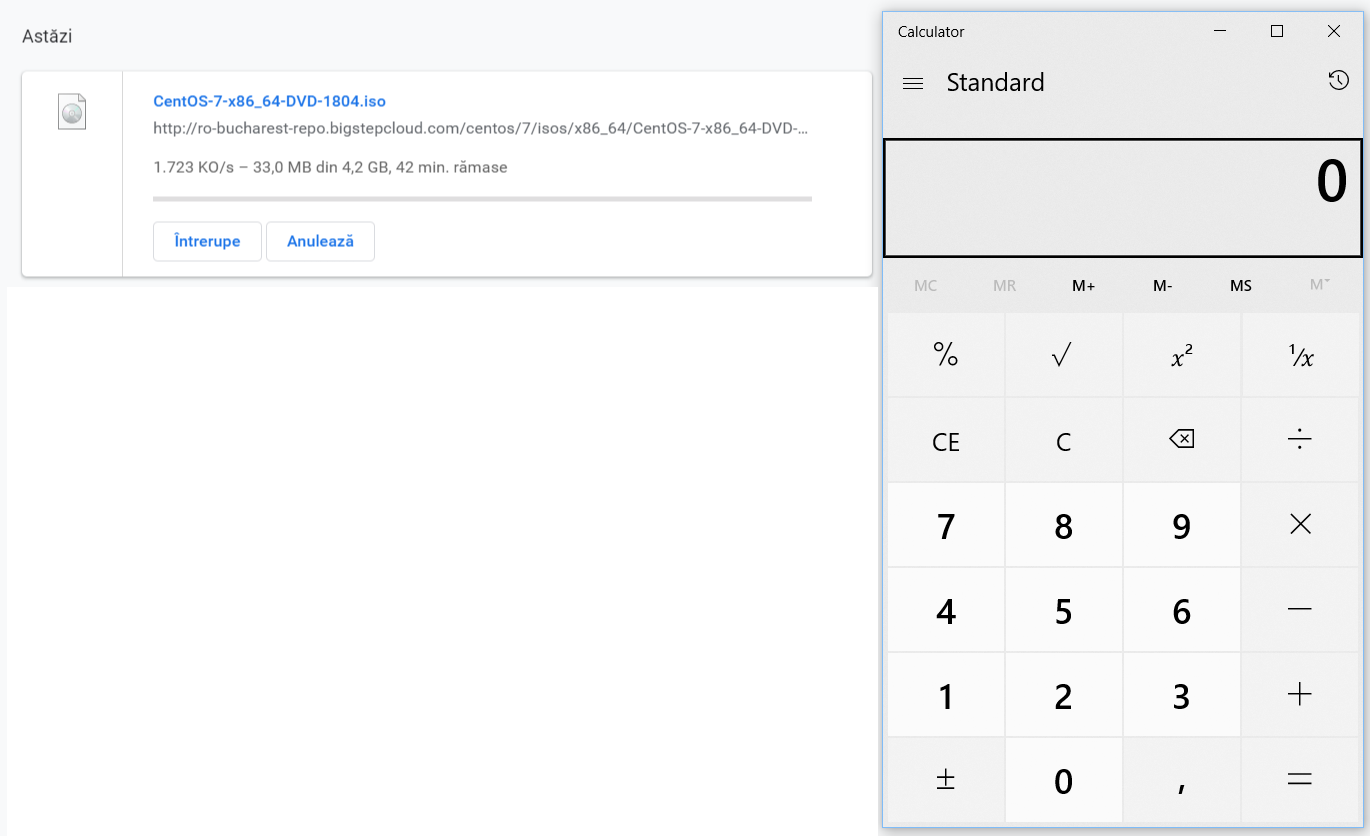
\includegraphics[width=15cm]{chapters/10-storage/img/concurrent-img.png}
  \caption{Executarea concomitentă a transferului de date și a unei aplicații}
  \label{fig:storage:concurrent-access}
\end{figure}

\section{Tipuri de discuri}
\label{sec:storage:type}

Subsistemul de stocare din cadrul unui sistem de calcul este format dintr-un controller care furnizează partea de logică a transferului de date și de unul sau mai multe discuri care stochează efectiv informația.
Dispozitivele de stocare au următoarele atribute principale:

\begin{itemize}
  \item spațiul disponibil - câtă informație se poate stoca pe disc (măsurat de obicei în gigabytes - GB sau terabytes - TB)
  \item viteza de acces - cât de repede se pot transfera datele de pe disc în memoria RAM (măsurat de obicei în megabytes pe secundă - MB/s)
  \item mod de poziționare - intern (în interiorul unității) sau extern (în exteriorul unității)
  \item mod de conectare - există două tipuri de conectare pentru discurile interne (SATA vs. SAS) și un tip de conectare pentru cele externe (USB)
  \item fiabilitate - câte ore de funcționare sau câte citiri/scrieri suportă de-a lungul vieții de funcționare.
    Aceste numere variază mult în funcție de tipul unității de stocare (HDD vs. SSD) și de gama pentru care a fost proiectat (folosirea în desktopuri vs. servere)
\end{itemize}

În zilele noastre există două tipuri de discuri pe sistemele de calcul:

\begin{itemize}
  \item \textit{Hard Disk Drive} (HDD)
  \item \textit{Solid State Drive} (SSD\abbrev{SSD}{Solid State Drive})
\end{itemize}

\subsection{Hard Disk Drive}
\label{sec:storage:type:hdd}

HDD-ul prin construcție dispune de părți mobile în interiorul acestuia: un braț de citire/scriere si unul sau mai multe platane pe care se stochează datele (vezi \labelindexref{Figura}{fig:storage:hdd}\footnote{\url{https://commons.wikimedia.org/wiki/File:Hard\_Drive\_(11644419853).jpg} (CC BY 2.0)}).
Astfel HDD-ul este predispus defectării atunci când acesta funcționează și este supus unor anumite șocuri mecanice.
De asemenea șocurile mecanice sunt problematice și atunci când HDD-ul nu funcționează (platanele nu se rotesc, iar capul de citire/scriere nu se mișcă).
Modelul constructiv al HDD-ului de asemenea nu permite viteze de funcționare ridicate comparativ cu memoria RAM.
Parametri prin care se măsoară performanța unui HDD sunt: numărul de rotații pe minut al platanelor și viteza interfeței de conectare la controller în gigabiți pe secundă.
În zilele noastre, există două tipuri de interfețe de conectare:

\begin{itemize}
  \item SATA - Serial ATA \abbrev{SATA}{Serial Advanced Technology Attachment} (\textit{Serial Advanced Technology Attachment})
  \item SAS - Serial Attached SCSI \abbrev{SAS}{Serial attached SCSI} (sau \textit{Serial Attached Small Computer System Interface})
\end{itemize}

\begin{figure}[!htbp]
  \centering
  \includegraphics[width=8cm]{chapters/10-storage/img/hdd-img.png}
  \caption{HDD}
  \label{fig:storage:hdd}
\end{figure}

În funcție de aceste interfețe se clasifică și discurile.
Ambele interfețe se interconectează cu controllerul la o viteză uzuală de 6Gbps.
Discurile cu interfețe de tip SATA au viteza de rotație mai redusă decât SAS (5400rpm/7200rpm vs. 10000rpm/15000rpm), iar durata de viață, din construcție, este mult mai mică decât a SAS-urilor.
De aceea discurile SATA sunt cu mult mai ieftine decât discurile SAS de aceeași capacitate (în cele mai multe cazuri pentru aceeași capacitate prețul se dublează).
Un alt deziderat al discurilor SATA este acela că se concentrează pe capacitatea de stocare, iar discurile SAS se concentrează pe viteza de funcționare.
Din cauza prețului foarte ridicat al discurilor SAS, acestea se folosesc în servere și sisteme de tip enterprise, iar discurile SATA se folosesc în calculatoarele personale.

În \labelindexref{Figura}{fig:storage:sas-sata}\footnote{\url{https://commons.wikimedia.org/wiki/File:SASvsSATA\_Connector.JPG} (CC BY-SA 3.0)} sunt reprezentate cele 2 tipuri de interfețe: în stânga sunt interfețe de tip SAS, iar în dreapta de tip SATA.

\begin{figure}[!htbp]
  \centering
  \includegraphics[width=8cm]{chapters/10-storage/img/sas-sata-img.png}
  \caption{SAS vs SATA}
  \label{fig:storage:sas-sata}
\end{figure}

\begin{figure}[!htbp]
  \centering
  \includegraphics[width=8cm]{chapters/10-storage/img/size-comp-img.png}
  \caption{2.5" vs 3.5"}
  \label{fig:storage:size-comp}
\end{figure}

O altă clasificare a discurilor este legată de mărimea fizică a acestora:

\begin{itemize}
  \item 2.5 inch (discurile din partea de sus din \labelindexref{Figura}{fig:storage:size-comp}\footnote{\url{https://commons.wikimedia.org/wiki/File:Comparison\_of\_3.5\_and\_2.5\_inch\_hard\_drives.jpg} (CC BY-SA 3.0)})
  \item 3.5 inch (discurile din partea de jos din \labelindexref{Figura}{fig:storage:size-comp})
\end{itemize}

Discurile de 2.5 inch se folosesc de obicei în sisteme enterprise, unde se dorește economisirea spațiului sau acomodarea a cât mai multe HDD-uri într-o unitate de rack (1U).

\subsection{SSD}
\label{sec:storage:type:ssd}

SSD-ul a venit ca un răspuns la neajunsurile HDD-ului, încercând să îmbunătățească sensibilitatea la șocuri și viteza de funcționare a acestuia.
SSD-ul nu are părți mobile în interiorul acestuia și funcționează pe principiul stickurilor USB: pentru a stoca informația se folosesc chipuri construite din semiconductoare și nu discuri/platane magnetice care prezintă o mișcare pentru a putea citi/scrie datele.

Discurile de tip SSD pot fi conectate atât printr-o interfață SATA ce oferă viteze de până la 6Gbps cât și printr-o interfață SAS ce oferă viteze de până la 12Gbps în acest moment.
Forma constructivă a unui SSD este de 2.5 inch sau de 3.5 inch, similar HDD-urilor.

Costul SSD-urilor comparativ cu cel al HDD-urilor, în special la capacități de peste 1TB este semnificativ mai mare (de aproximativ 5 ori).
De aceea, în unele dintre sistemele din ziua de astăzi există un disc principal SSD, unde se stochează sistemul de operare și aplicațiile care au nevoie de acces rapid, și un HDD de mare capacitate, pentru stocarea datelor de termen lung și care nu necesită viteză ridicată.

Un aspect de luat în considerare atunci când se achiziționează un disc de tip SSD este durata de viață.
Spre deosebire de un HDD, SSD-ul are un număr limitat de scrieri specificat de producător, după care se spune că s-a finalizat durata de viață a acestuia.
Din acest motiv, sistemele de operare și sistemul de fișiere întreprind operații specifice, optimizate pentru SSD-uri, pentru a le prelungi durata de viață (de exemplu, defragmentarea generează foarte multe scrieri, scurtând durata de viață a discului, iar aceasta nu este utilă pentru un SSD - viteza de citire a oricăror date aleator de pe disc este aceeași în cazul SSD-urilor).
Pentru a afla durata de viață a unui disc SSD există utilitare speciale cum ar fi SSD Life\footnote{\url{https://ssd-life.com}}.

Pentru a prelungi durata de viață a unui disc, trebuie avute în vedere următoarele facilități:

\begin{itemize}
  \item defragmentarea (procesul prin care se rearanjează datele pe disc pentru un acces mai eficient) - este recomandată dezactivarea defragmentării pentru discurile SSD (dupa cum am specificat mai sus)
  \item swapping - atunci când un sistem rămâne fără memorie RAM, acesta va folosi pe post de memorie discul.
Este recomandat să dezactivați swappingul pe discurile SSD dacă doriți prelungirea duratei de viață (mai ales dacă swappingul apare des)
  \item hibernate - atunci când trecem calculatorul în starea Hibernate acesta scrie întregul conținut al memoriei pe disc (ceea ce va genera foarte multe scrieri).
Este recomandat să nu treceți sistemul în Hibernate dacă doriți prelungirea duratei de viață (sau să configurați un disc alternativ pentru Hibernate).
\end{itemize}

Alte recomandări pentru creșterea duratei de viață a discului SSD specifice sistemului de operare folosit, le puteți găsi la o simplă căutare pe Google\footnote{de ex. \url{https://www.makeuseof.com/tag/3-top-tips-maintain-performance-extend-life-ssd-si/}}.

\section{Partiționarea dispozitivelor de stocare}
\label{sec:storage:partition}

În secțiunile anterioare au fost prezentate caracteristicile discurilor SSD și HDD.
O caracteristică principală a acestora este capacitatea mare de stocare (mult mai care decât a memoriei RAM).
Așadar o adresare liniară nu este suficientă pentru a gestiona spațiul de stocare oferit de un disc.
Mai mult, un alt motiv este constituit de faptul că administrarea spațiului de stocare este făcută de către utilizator;
în schimb gestionarea zonei de memorie RAM este făcută de către sistemul de operare.
Astfel administrarea spațiului de stocare trebuie să fie simplă și facilă.

Spațiul de stocare oferit de un dispozitiv trebuie administrat în mod corect pentru a asigura o stocare eficientă (performanță ridicată) și coerentă (să nu corupem date).
Există două niveluri de administrare: partiționare și sistemele de fișiere.
Aceste niveluri sunt interdependente și se aplică iterativ.

Partiționarea împarte spațiul disponibil în zone continue fizic (numite \textbf{zone contigue}), fiecare zonă având un specific definit la creare (partiție de boot, partiție pentru utilizatori, partiție pentru sistemul de de operare).
Există două tipuri de partiționări în sistemele din ziua de astăzi, așa cum am prezentat în \labelindexref{Capitolul}{ch:boot}:

\begin{itemize}
  \item Master Boot Record (referit ca MBR) - acesta a fost introdus în 1983 și poartă această denumire deoarece stochează la începutul discului un sector specific procesului de bootare.
  \item GUID Partition Table (referit ca GPT) - este o metodă mai nouă de partiționare ce va înlocui treptat MBR din cauza limitărilor acestuia.
\end{itemize}

Schema MBR, după cum se menționează anterior, are alocat exact la începutul unui disc un sector special de boot care reține schema de partiționare precum și o versiune minimală a bootloaderului care va încărca sistemul de operare, așa cum am precizat în \labelindexref{Capitolul}{ch:boot}.
 Schema de partiționare MBR este formată din maxim 4 partiții, denumite \textbf{partiții primare}.
Pentru a acoperi aceste neajunsuri, au fost introduse \textbf{partițiile logice}: una din partițiile primare va fi alocată pe întreg discul rămas liber și va fi marcată ca \textbf{partiție extinsă}.
În cadrul partiției extinse se pot crea oricâte partiții logice se dorește.
Acest lucru îngreunează schema de partiționare, iar unele sisteme de operare nu pot porni folosind aceste partiții.
Nu se recomandă folosirea acestor partiții ca partiții de bootare.
Întreaga schemă de partiționare a MBR este descrisă și în \labelindexref{Figura}{fig:storage:mbr}.

\begin{figure}[htbp]
  \centering
  \def\svgwidth{\columnwidth}
  \includesvg{chapters/10-storage/img/mbr-struct.svg}
  \caption{Schema de partiționare a MBR}
  \label{fig:storage:mbr}
\end{figure}

MBR a început să fie înlocuit de către GPT din cauza limitărilor acestuia:

\begin{itemize}
  \item dimensiunea maximă a unei partiții este de 2TB
  \item necesitatea unei partiții extinse pentru a crea mai mult de patru partiții
\end{itemize}

Pentru a rezolva neajunsurile MBR, a fost creată schema de partiționare GPT.
Numele \textit{GUID Partition Table} (GPT) provine de la faptul că fiecare partiție a discului are asociat un număr unic de identificare (\textit{guid}\abbrev{GUID}{Globally Unique Identifier} - \textit{Globally Unique Identifier}), generat aleator și care garantează că fiecare partiție de pe glob va avea propriul identificator unic.

GPT este asociat în general cu standardul UEFI care dorește înlocuirea BIOS în sistemele de calcul, despre care am discutat în \labelindexref{Capitolul}{ch:boot}.
BIOS și UEFI sunt componente low-level care se execută la pornirea sistemelor de calcul pentru a realiza testarea și inițializarea componentelor.
UEFI este un nou standard, menit să înlocuiască BIOS pentru a acoperi neajunsurile acestuia.

În \labelindexref{Figura}{fig:storage:gpt} este reprezentată schema de partiționare GPT.
Se observă asemănarea cu partiționarea de tip MBR: la începutul discului există sectorul de boot.
După sectorul de boot se află headerul GPT ce descrie partițiile (maxim 128).
Sectorul de boot și header sunt duplicate și la finalul discului: în caz de corupere a primelor sectoare să nu pierdem detaliile despre schema de partiționare.
În cazul GPT nu mai avem limitarea la 2TB a unei partiții și nici limitarea la 4 partiții primare (din cauza numărului ridicat disponibil de partiții nu mai există noțiunea de partiții logice).

\begin{figure}[htbp]
  \centering
  \def\svgwidth{\columnwidth}
  \includesvg[width=0.7\textwidth]{chapters/10-storage/img/gpt-struct.svg}
  \caption{Schema de partiționare a GPT}
  \label{fig:storage:gpt}
\end{figure}

Pentru a utiliza spațiul de stocare eficient, există recomandări din partea vendorilor sistemelor de operare.
Bunele practici în partiționarea unui disc includ:

\begin{itemize}
  \item Crearea unei partiții de boot (specific Linux \file{/boot} - conține nucleul sistemului de operare și bootloaderul)
  \item Crearea unei partiții de swap (specific Linux - spațiu utilizat de sistemul de operare atunci când rămâne fără memorie;
în cazul Windows swap-ul este alocat din partiția sistemului de operare)
  \item Crearea unei partiții pentru sistemul de operare (pentru Linux este \file{/}, denumită și partiția rădăcină - \textit{root partition}, iar pentru Windows de obicei este discul \file{C:})
  \item Crearea unei partiții pentru utilizatorii sistemului - atunci când reinstalăm sistemul de operare, să putem păstra ușor datele utilizatorilor (pentru Linux este \file{/home}, iar pentru Windows de obicei literele de la \file{D:} în sus)
  \item Crearea unei partiții pentru sistemele cu suport EFI/UEFI (specific Linux în \file{/boot/efi} și conține fișierele necesare să fie executate la încărcarea sistemului de operare de către subsistemul UEFI)
\end{itemize}

Utilitare ce pot fi folosite pentru administrarea partițiilor sunt:

\begin{itemize}
  \item Pentru Linux: \cmd{fdisk} (doar MBR), \cmd{gdisk} (pentru GPT);
    \cmd{parted}/\cmd{gparted} (suport extins pentru MBR/GPT și operații avansate).
    O dată creată o partiție, aceasta poate fi văzută în calea \file{/dev} și poartă numele discului partiționat (ex. \texttt{sda}) urmat de o cifră care reprezintă numărul partiției (ex. \texttt{sda5})
  \item Pentru Windows: \cmd{Disk Management}.
    O data creată o partiție, aceasta poate fi văzută în utilitarul menționat.
\end{itemize}

\subsection{Sisteme de fișiere}
\label{sec:storage:fs}

Pentru a putea organiza datele pe o partiție într-un mod facil și ușor de înțeles pentru utilizatorul final al sistemului de calcul, pe aceasta în general se instalează un sistem de fișiere.
Procesul de instalare/alocare a unui sistem de fișiere pe o partiție se numește \textbf{formatare}.
O partiție fără un sistem de fișiere nu poate fi utilizată/explorată de către utilizatorul final.
De exemplu, în Windows, un disc USB neformatat nu va putea fi accesat cu dublu-click și va apărea un mesaj către utilizator dacă acceptă formatarea lui ca în \labelindexref{Figura}{fig:storage:format-disk}.

\begin{figure}[!htbp]
  \centering
  \includegraphics[width=8cm]{chapters/10-storage/img/format-disk-img.png}
  \caption{Fereastră privind formatarea unui disc în Windows}
  \label{fig:storage:format-disk}
\end{figure}

Sistemul de fișiere oferă următoarele obiecte vizibile utilizatorului final:

\begin{itemize}
  \item fișierul - entitatea care conține date utile în diverse formate
  \item directorul - entitatea care organizează fișierele într-un formă arborescentă ușor de folosit de către utilizator
\end{itemize}

Mai multe detalii legate de fișiere și directoare (modul în care se creează, se șterg, permisiuni de acces) se găsesc în \labelindexref{Capitolul}{ch:fs}.

În general sistemele de fișiere sunt specifice sistemelor de operare.
Astfel avem următoarea clasificare:

\begin{itemize}
  \item Linux: cel mai folosit este sistemul de fișiere Ext4, iar mai nou acesta ajunge să fie înlocuit cu XFS
  \item Windows: principalul sistem de fișiere este NTFS
\end{itemize}

În Linux, pentru a formata (instala) un sistem de fișiere pe o partiție se folosește comandă \cmd{mkfs} urmată de sufixul sistemului de operare dorit și partiția dorită (ex. \cmd{mkfs.ext4 /dev/sda2}).
\textbf{Atenție}: procesul de formatare a unui sistem de fișiere distruge datele prezente pe acea partiție.
O greșeală frecventă este aplicarea procesului de formatare pe întreg discul (ex. \cmd{mkfs.ext4 /dev/sda}).
Acest lucru va șterge \textbf{toate} partițiile de pe acel disc.
Un exemplu complet de folosire a utilitarelor de formatare și partiționare îl puteți găsi la finalul capitolului, la studii de caz.

\begin{figure}[!htbp]
  \centering
  \includegraphics[width=8cm]{chapters/10-storage/img/format-part-img.png}
  \caption{Formatarea unei partiții în Windows}
  \label{fig:storage:win-format}
\end{figure}

În Windows, pentru a formata (instala) un sistem de fișiere pe o partiție, se face click dreapta pe litera aferentă partiției și există opțiunea \texttt{Format}: de aici se poate selecta tipul sistemului de fișiere și diverse caracteristici de formatare, ca în \labelindexref{Figura}{fig:storage:win-format}.

Pentru a putea folosi un sistem de fișiere, acesta trebuie făcut disponibil utilizatorului.
Procesul prin care acest este disponibil pentru citire/scriere se numește \textbf{montare}.

Pe sistemele bazate pe Linux, montarea se realizează cu comanda \cmd{mount} urmată de partiția care se dorește a fi montată și directorul unde să fie montată în sistemul de fișiere (numit punct de montare - \textit{mount point}):

\begin{screen}
student@uso:~$ sudo mount /dev/sdb2 /mnt/sdb2
student@uso:~$ mount
[...]
/dev/sdb2 on /mnt/sdb2 type ext4 (rw,relatime,data=ordered)
\end{screen}

Demontarea se face cu ajutorul comenzii \cmd{umount}:

\begin{screen}
student@uso:~$ sudo umount /mnt/sdb2
\end{screen}

Un lucru specific sistemelor de operare bazate pe Linux este alocarea unui identificator la formatarea unei partiții, numit UUID (\textit{Universally Unique Identifier}).
Astfel la montare se poate specifica identificatorul partiției în loc calea către dispozitiv.
Acest lucru este utilizat pentru a rezolva conflictele generate de schimbarea ordinii discurilor fizice.
De exemplu, în cazul prezentat mai sus, dacă mai inserăm un disc fizic în sistem, acesta poate fi detectat înainte celui prezent și i se va aloca litera \texttt{b}, deci va fi \texttt{sdb}, iar cel curent va deveni \texttt{sdc}.
Astfel comanda de mai sus devine invalidă și inconsistentă deoarece va monta un cu totul alt disc.
Pentru a afla UUID-ul alocat unei partiții noi formatate se folosește comanda \cmd{blkid}:

\begin{screen}
student@uso:~$ sudo blkid /dev/sdb2
/dev/sdb2: UUID="6ea1370c-b47c-497f-a7b7-556d40d4af97" TYPE="ext4" PARTUUID="f3aa63a6-02"
\end{screen}

Acum putem monta partiția folosind UUID-ul:

\begin{screen}
student@uso:~$ sudo mount -U 6ea1370c-b47c-497f-a7b7-556d40d4af97 /mnt/sdb2
student@uso:~$ mount
[...]
/dev/sdb2 on /mnt/sdb2 type ext4 (rw,relatime,data=ordered)
\end{screen}

În Windows montarea se realizează în general automat de către sistemul de operare.
Dacă se doresc operații avansate, acestea pot fi făcute tot din \textit{Disk Management}: \texttt{Start $\rightarrow$ Run $\rightarrow$ diskmgmt.msc}, ca în \labelindexref{Figura}{fig:storage:win-disk-manage}.

\begin{figure}[!htbp]
  \centering
  \includegraphics[width=0.6\textwidth]{chapters/10-storage/img/admin-img.png}
  \caption{Administrarea spațiului de stocare în Windows}
  \label{fig:storage:win-disk-manage}
\end{figure}

Anterior, s-a menționat faptul că sistemele de fișiere sunt specifice sistemului de operare.
La nevoie, aceste sisteme de fișiere se pot monta pe alt sistem de operare decât cele pentru care au fost proiectate.
Acest lucru nu este întotdeauna recomandat întrucât există penalizări de performanță și risc de corupere a datelor.

Sistemele de fișiere au mecanisme interne de recuperare a datelor corupte.
 Principalul mecanism prin care se realizează acest lucru este jurnalizarea (\textit{file system journal}).
Fiecare sistem de fișiere scrie fiecare operație adusă sistemului de fișiere într-un jurnal.
Atunci când sunt probleme la montarea unui sistem de fișiere, acesta folosește jurnalul pentru a încerca să repare problemele de coerență a datelor.
De multe ori nu se poate monta sistemul de fișiere fără o verificare completă a integrității sistemului de fișiere.
Acest lucru se realizează de obicei automat la pornirea sistemului de operare, atât în Linux cât și în Windows.
Este important de menționat faptul că nu toate sistemele de fișiere oferă suport de jurnalizare.
În ziua de astăzi, anumite sisteme de fișiere simple nu oferă acest suport;
sunt simple și se adresează dispozitivelor specializate (ex. camere video) și cu puține resurse care nu au implementat un mecanism de verificare a integrității;
un astfel de sisteme de fișiere este FAT.

În Linux, dacă este necesară verificarea integrității sistemului de fișiere manual, se poate folosi utilitarul \cmd{fsck}, ca în \labelindexref{Listing}{lst:storage:fsck}.
 Se observă că nu se poate verifica sistemul de fișiere când acesta este deja montat.
Vom demonta sistemul de fișiere iar apoi vom verifica integritatea.

\begin{screen}[caption={Verificarea integrității sistemului de fișiere},label={lst:storage:fsck}]
student@uso:~$ sudo fsck /dev/sdb2
fsck from util-linux 2.31.1
e2fsck 1.44.1 (24-Mar-2018)
/dev/sdb2 is mounted.
e2fsck: Cannot continue, aborting.

student@uso:~$ sudo umount /dev/sdb2
student@uso:~$ sudo fsck /dev/sdb2
fsck from util-linux 2.31.1
e2fsck 1.44.1 (24-Mar-2018)
/dev/sdb2: clean, 11/51296 files, 7726/204800 blocks
\end{screen}

Ca și schemele de partiționare, sistemele de fișiere au și ele anumite limitări legate de:

\begin{itemize}
  \item numărul maxim de fișiere (ex. pentru ext4 - 4 miliarde)
  \item dimensiunea partiției (ex. pentru ext4 - 1024PB)
  \item dimensiunea maximă a fișierului (ex. pentru ext4 - 16TB)
  \item atribute extinse de funcționalitate și securitate
\end{itemize}

Limitările menționate mai sus variază de la un sistem de operare la altul, sunt precizate în documentația respectivului sistem de fișiere.

Până în acest punct am discutat despre disc și partiție.
Discul este partea fizică a sistemului de calcul disponibilă spre a fi folosită de către sistemul de operare.
Pentru o folosire eficientă, acesta este partiționat (partiție).
 Deseori, prin diverse tehnici (RAID hardware sau software), mai multe discuri sunt puse la comun și văzute ca unul singur.
 Rezultatul poartă numele de \textit{volum}.
Un alt termen folosit în administrarea spațiului de stocare este \textit{drive}.
Acesta are două semnificații: referă tot un disc fizic sau referă o partiție pe sisteme Windows.

\section{Anexă: Adăugarea unui disc mașinii virtuale}
\label{sec:storage:vm-disk}

Pentru partea demonstrativă a acestui capitol, folosim un disc nou adăugat mașinii virtuale.
 Acest disc va fi vizibil în sistemul de operare (Linux) al mașinii virtuale ca \file{/dev/sdb}.
Spunem că discul este un disc virtual.

Pentru a adăuga un disc mașinii virtuale USO și, în general, pentru a adăuga un disc nou unei mașini virtuale VirtualBox, se urmează pașii:
\begin{enumerate}
  \item click dreapta pe intrarea mașinii virtuale în VirtualBox și deschiderea meniului contextual
  \item selectarea opțiunii \texttt{Settings} din meniul contextual deschis
  \item în fereastra nou deschisă (\texttt{Settings}), navigarea la intrarea \texttt{Storage}
  \item în noul ecran se folosește iconul \texttt{Adds hard disk} pentru adăugarea unui nou disc la controllerul SATA, ca în \labelindexref{Figura}{fig:storage:vm-new-disk}
  \item se selectează în ordine \texttt{Create new disk}, \texttt{VDI}, \texttt{Dynamically allocated}
  \item se alege un nume și o dimensiune;
    de exemplu, pentru partea demonstrativă a acestui capitol, am ales numele \texttt{my.vdi} și dimensiunea de \texttt{2GB} ca în \labelindexref{Figura}{fig:storage:vm-disk-info}
\end{enumerate}

În acest moment avem un nou disc în cadrul mașinii virtuale.
 În interfața VirtualBox, din \labelindexref{Figura}{fig:storage:vm-disk-info}, discul este văzut ca \texttt{my.vdi}.
 În sistemul de operare Linux din mașina virtuală, discul va apărea ca \file{/dev/sdb}.

\begin{figure}[!htbp]
  \centering
  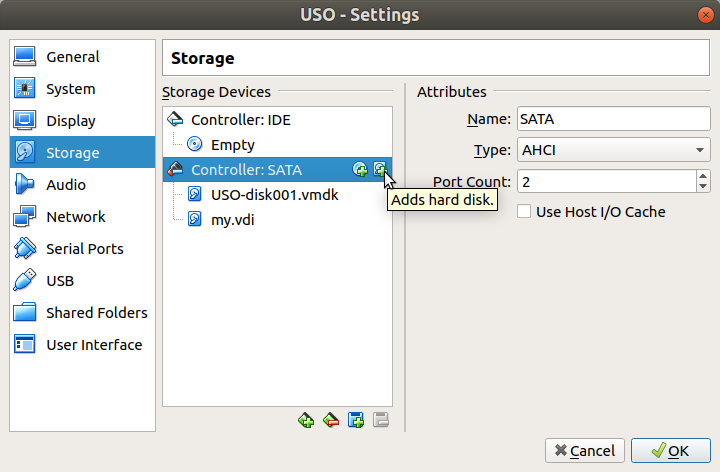
\includegraphics[width=0.6\textwidth]{chapters/10-storage/img/vm-new-disk.png}
  \caption{Adăugarea unui nou disc mașinii virtuale}
  \label{fig:storage:vm-new-disk}
\end{figure}

\begin{figure}[!htbp]
  \centering
  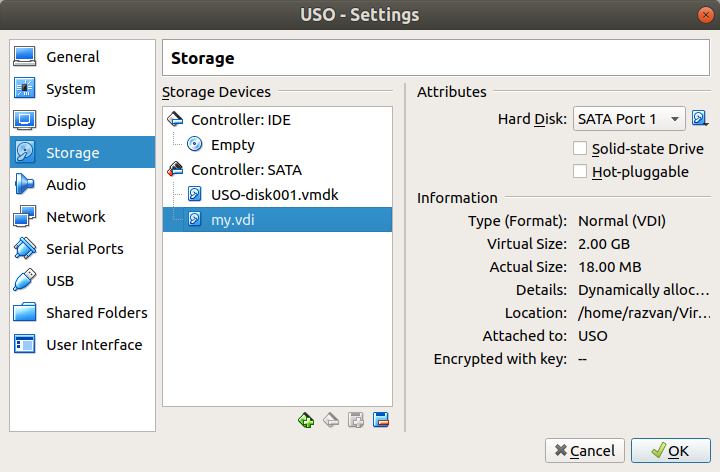
\includegraphics[width=0.6\textwidth]{chapters/10-storage/img/vm-disk-info.png}
  \caption{Informații despre un disc virtual}
  \label{fig:storage:vm-disk-info}
\end{figure}

\section{Anexă: Investigarea spațiului de stocare}
\label{sec:storage:investigate-cmd}

În Linux, pentru a vizualiza toate discurile din sistem, precum și unde sunt montate, putem folosi utilitarul \cmd{lsblk} ca în \labelindexref{Listing}{lst:storage:lsblk}.
 Există două discuri în sistem (\texttt{sda} și \texttt{sdb}) și un dispozitiv de tip CD ROM (\texttt{sr0}).
 Discul \texttt{sda} are o partiție (\texttt{sda1}) care ocupă tot discul (\texttt{16GB}).

\begin{screen}[caption={Afișarea discurilor din sistem (lsblk)},label={lst:storage:lsblk}]
student@uso:~$ lsblk -i
NAME   MAJ:MIN RM   SIZE RO TYPE MOUNTPOINT
[...]
sda      8:0    0    16G  0 disk
`-sda1   8:1    0    16G  0 part /
sdb      8:16   0     2G  0 disk
sr0     11:0    1  1024M  0 rom
\end{screen}

Informații despre partițiile montate ale sistemului și spațiul ocupat de acestea pot fi vizualizate folosind utilitarul \cmd{df} ca în \labelindexref{Listing}{lst:storage:df}.
 Opțiunea \texttt{-h} este folosită pentru a afișa dimensiunea partițiilor în format ușor de citit -- \textit{human readable}:

\begin{screen}[caption={Informații despre partiții montate (df)},label={lst:storage:df}]
student@uso:~$ df -h
Filesystem      Size  Used Avail Use% Mounted on
[...]
/dev/sda1        16G   11G  4.2G  73% /
[...]
\end{screen}

Pentru a putea investiga spațiul ocupat de un anumit fișier sau director, putem folosi comanda \cmd{du} ca în \labelindexref{Listing}{lst:storage:du}.
 Opțiunea \texttt{-h} este folosită pentru a afișa dimensiunea în format ușor de citit, iar \texttt{-s} realizează sumarizarea tuturor fișierelor din acel director.
Dacă nu folosim opțiunea \texttt{-s}, atunci ni se va afișa fiecare fișier recursiv al acelui director.

\begin{screen}[caption={Informații despre spațiul ocupat de directoare (du)},label={lst:storage:du}]
student@uso:~$ du -hs /opt
95M	/opt

student@uso:~$ du -h /opt
52K	/opt/VBoxGuestAdditions-5.2.18/init
4.7M	/opt/VBoxGuestAdditions-5.2.18/lib
1.8M	/opt/VBoxGuestAdditions-5.2.18/other
1.5M	/opt/VBoxGuestAdditions-5.2.18/bin
288K	/opt/VBoxGuestAdditions-5.2.18/src/vboxguest-5.2.18/vboxvideo
40K	/opt/VBoxGuestAdditions-5.2.18/src/vboxguest-5.2.18/vboxguest/common/err
176K	/opt/VBoxGuestAdditions-5.2.18/src/vboxguest-5.2.18/vboxguest/common/log
40K	/opt/VBoxGuestAdditions-5.2.18/src/vboxguest-5.2.18/vboxguest/common/alloc
172K	/opt/VBoxGuestAdditions-5.2.18/src/vboxguest-5.2.18/vboxguest/common/string
96K	/opt/VBoxGuestAdditions-5.2.18/src/vboxguest-5.2.18/vboxguest/common/misc
[...]
\end{screen}

Pentru a investiga informații despre partițiile unui disc se folosesc utilitarele \cmd{fdisk} (pentru partiții MBR), \cmd{gdisk} (pentru partiții GPT) sau \cmd{parted}/\cmd{gparted}.
Comanda \cmd{fdisk -l} va lista toate discurile și partițiile unui sistem, ca în \labelindexref{Listing}{lst:storage:fdisk-list}.
 Dacă se adaugă un parametru suplimentar (calea către discul pe care se dorește a fi inspectat), atunci doar acesta va fi afișat.
 Informațiile despre partiții sunt informații critice din sistem, așa că rularea trebuie făcut în mod privilegiat, prin prefixarea comenzii cu \cmd{sudo}.

\begin{screen}[caption={Afișarea partițiilor (fdisk)},label={lst:storage:fdisk-list}]
student@uso:~$ sudo fdisk -l
[...]
Disk /dev/sda: 16 GiB, 17179869184 bytes, 33554432 sectors
Units: sectors of 1 * 512 = 512 bytes
Sector size (logical/physical): 512 bytes / 512 bytes
I/O size (minimum/optimal): 512 bytes / 512 bytes
Disklabel type: dos
Disk identifier: 0xdf4f561b

Device     Boot Start      End  Sectors Size Id Type
/dev/sda1  *     2048 33552383 33550336  16G 83 Linux

Disk /dev/sdb: 2 GiB, 2147483648 bytes, 4194304 sectors
Units: sectors of 1 * 512 = 512 bytes
Sector size (logical/physical): 512 bytes / 512 bytes
I/O size (minimum/optimal): 512 bytes / 512 bytes

student@uso:~$ sudo fdisk -l /dev/sda
Disk /dev/sda: 16 GiB, 17179869184 bytes, 33554432 sectors
Units: sectors of 1 * 512 = 512 bytes
Sector size (logical/physical): 512 bytes / 512 bytes
I/O size (minimum/optimal): 512 bytes / 512 bytes
Disklabel type: dos
Disk identifier: 0xdf4f561b

Device     Boot Start      End  Sectors Size Id Type
/dev/sda1  *     2048 33552383 33550336  16G 83 Linux
\end{screen}

Dacă renunțăm la parametrul \texttt{-l}, vom intra în modul interactiv al utilitarului \cmd{fdisk}, ca în \labelindexref{Listing}{lst:storage:fdisk-interact}.
 Forma interactivă a utilitarului va afișa un prompt unde se vor introduce comenzi.
 În \labelindexref{Listing}{lst:storage:fdisk-interact} sunt folosite două comenzi:

\begin{itemize}
  \item comanda \texttt{m}: este comanda de ajutor care afișează comenzile disponibile
  \item comanda \texttt{p}: afișează tabela de partiții a discului investigat
  \item comanda \texttt{q}: închide aplicația interactivă \cmd{fdisk}
\end{itemize}

\begin{screen}[caption={Mod interactiv pentru fdisk},label={lst:storage:fdisk-interact}]
student@uso:~$ sudo fdisk /dev/sda
[...]
Command (m for help): m

Help:

  DOS (MBR)
   a   toggle a bootable flag
   b   edit nested BSD disklabel
   c   toggle the dos compatibility flag

  Generic
   d   delete a partition
   F   list free unpartitioned space
   l   list known partition types
   n   add a new partition
   p   print the partition table
   t   change a partition type
   v   verify the partition table
   i   print information about a partition

  Misc
   m   print this menu
   u   change display/entry units
   x   extra functionality (experts only)

  Script
   I   load disk layout from sfdisk script file
   O   dump disk layout to sfdisk script file

  Save & Exit
   w   write table to disk and exit
   q   quit without saving changes

  Create a new label
   g   create a new empty GPT partition table
   G   create a new empty SGI (IRIX) partition table
   o   create a new empty DOS partition table
   s   create a new empty Sun partition table


Command (m for help): p
Disk /dev/sda: 16 GiB, 17179869184 bytes, 33554432 sectors
Units: sectors of 1 * 512 = 512 bytes
Sector size (logical/physical): 512 bytes / 512 bytes
I/O size (minimum/optimal): 512 bytes / 512 bytes
Disklabel type: dos
Disk identifier: 0xdf4f561b

Device     Boot Start      End  Sectors Size Id Type
/dev/sda1  *     2048 33552383 33550336  16G 83 Linux

Command (m for help): q

student@uso:~$
\end{screen}

Utilitarul \cmd{parted} se folosește în mod asemănător cu \cmd{fdisk}.
 Pentru a administra un disc în mod interactiv se rulează comanda \cmd{parted} urmată de calea către dispozitiv, ca în \labelindexref{Listing}{lst:storage:parted}.
 Similar \cmd{fdisk}, forma interactivă a utilitarului \cmd{parted} primește comenzi:

\begin{itemize}
  \item \texttt{help}: afișează un sumar al comenzilor disponibile
  \item \texttt{p} / \texttt{print}: afișează tabela de partiții a discului
  \item \texttt{q} / \texttt{quit}: închide aplicația interactivă
\end{itemize}

\begin{screen}[caption={Gestiunea discurilor folosind parted},label={lst:storage:parted}]
student@uso:~$ sudo parted /dev/sda
GNU Parted 3.2
Using /dev/sda
Welcome to GNU Parted! Type 'help' to view a list of commands.
(parted) help
  align-check TYPE N                        check partition N for TYPE(min|opt) alignment
  help [COMMAND]                           print general help, or help on COMMAND
  mklabel,mktable LABEL-TYPE               create a new disklabel (partition table)
  mkpart PART-TYPE [FS-TYPE] START END     make a partition
  name NUMBER NAME                         name partition NUMBER as NAME
  print [devices|free|list,all|NUMBER]     display the partition table, available devices, free space, all found partitions, or a particular partition
  quit                                     exit program
  rescue START END                         rescue a lost partition near START and END
  resizepart NUMBER END                    resize partition NUMBER
  rm NUMBER                                delete partition NUMBER
  select DEVICE                            choose the device to edit
  disk_set FLAG STATE                      change the FLAG on selected device
  disk_toggle [FLAG]                       toggle the state of FLAG on selected device
  set NUMBER FLAG STATE                    change the FLAG on partition NUMBER
  toggle [NUMBER [FLAG]]                   toggle the state of FLAG on partition NUMBER
  unit UNIT                                set the default unit to UNIT
  version                                  display the version number and copyright information of GNU Parted
(parted) p
Model: ATA VBOX HARDDISK (scsi)
Disk /dev/sda: 17.2GB
Sector size (logical/physical): 512B/512B
Partition Table: msdos
Disk Flags:

Number  Start   End     Size    Type     File system  Flags
 1      1049kB  17.2GB  17.2GB  primary  ext4         boot

(parted) q

student@uso:~$
\end{screen}

\section{Anexă: Partiționare, formatare și montare în Linux}
\label{sec:storage:partition-cmd}

Vom realiza pas cu pas partiționarea, formatarea și montarea unui disc în Linux.
Vom realiza partiționarea discului folosind forma interactivă a utilitarului \cmd{fdisk}.
Vom realiza formatarea partițiilor folosind utilitarele din familia \cmd{mkfs}.
Vom monta partițiile folosind utilitarul \cmd{mount}.

Partiționarea discului este prezentată în \labelindexref{Listing}{lst:storage:partition-fdisk}.
În rularea interactivă a utilitarului \cmd{fdisk} am folosit comenzile:
\begin{itemize}
  \item \texttt{p}: afișarea tabelei de partiții
  \item \texttt{n}: crearea unei partiții noi.
    Când creăm o partiție nouă, intrăm într-un submod interactiv în care precizăm tipul partiției (primară sau logică), indexul ei, și începutul și sfârșitul (în număr de sector)
  \item \texttt{w}: scrierea tabelei de partiții pe disc;
    permanentizarea modificărilor
\end{itemize}

În urma comenzilor din \labelindexref{Listing}{lst:storage:partition-fdisk} am creat trei partiții primare: \texttt{sdb1} (\texttt{500MB}), \texttt{sdb2} (\texttt{800MB}) și \texttt{sdb3} (\texttt{747MB}).
Pentru afișarea partițiilor am folosit comanda \texttt{p} din rularea interactivă a utilitarului \cmd{fdisk} și opțiunea \texttt{-l} la rularea neinteractivă.

\begin{screen}[caption={Partiționarea unui disc folosind fdisk},label={lst:storage:partition-fdisk}]
student@uso:~$ sudo fdisk /dev/sdb

Welcome to fdisk (util-linux 2.31.1).
Changes will remain in memory only, until you decide to write them.
Be careful before using the write command.

Device does not contain a recognized partition table.
Created a new DOS disklabel with disk identifier 0xf3aa63a6.

Command (m for help): p
Disk /dev/sdb: 2 GiB, 2147483648 bytes, 4194304 sectors
Units: sectors of 1 * 512 = 512 bytes
Sector size (logical/physical): 512 bytes / 512 bytes
I/O size (minimum/optimal): 512 bytes / 512 bytes
Disklabel type: dos
Disk identifier: 0xf3aa63a6

Command (m for help): n
Partition type
   p   primary (0 primary, 0 extended, 4 free)
   e   extended (container for logical partitions)
Select (default p): p
Partition number (1-4, default 1):
First sector (2048-4194303, default 2048):
Last sector, +sectors or +size{K,M,G,T,P} (2048-4194303, default 4194303): +500M

Created a new partition 1 of type 'Linux' and of size 500 MiB.

Command (m for help): n
Partition type
   p   primary (1 primary, 0 extended, 3 free)
   e   extended (container for logical partitions)
Select (default p): p
Partition number (2-4, default 2):
First sector (1026048-4194303, default 1026048):
Last sector, +sectors or +size{K,M,G,T,P} (1026048-4194303, default 4194303): +800M

Created a new partition 2 of type 'Linux' and of size 800 MiB.

Command (m for help): n
Partition type
   p   primary (2 primary, 0 extended, 2 free)
   e   extended (container for logical partitions)
Select (default p): p
Partition number (3,4, default 3):
First sector (2664448-4194303, default 2664448):
Last sector, +sectors or +size{K,M,G,T,P} (2664448-4194303, default 4194303):

Created a new partition 3 of type 'Linux' and of size 747 MiB.

Command (m for help): p
Disk /dev/sdb: 2 GiB, 2147483648 bytes, 4194304 sectors
Units: sectors of 1 * 512 = 512 bytes
Sector size (logical/physical): 512 bytes / 512 bytes
I/O size (minimum/optimal): 512 bytes / 512 bytes
Disklabel type: dos
Disk identifier: 0xf3aa63a6

Device     Boot   Start     End Sectors  Size Id Type
/dev/sdb1          2048 1026047 1024000  500M 83 Linux
/dev/sdb2       1026048 2664447 1638400  800M 83 Linux
/dev/sdb3       2664448 4194303 1529856  747M 83 Linux

Command (m for help): w
The partition table has been altered.
Calling ioctl() to re-read partition table.
Syncing disks.

student@uso:~$ sudo fdisk -l /dev/sdb
Disk /dev/sdb: 2 GiB, 2147483648 bytes, 4194304 sectors
Units: sectors of 1 * 512 = 512 bytes
Sector size (logical/physical): 512 bytes / 512 bytes
I/O size (minimum/optimal): 512 bytes / 512 bytes
Disklabel type: dos
Disk identifier: 0xf3aa63a6

Device     Boot   Start     End Sectors  Size Id Type
/dev/sdb1          2048 1026047 1024000  500M 83 Linux
/dev/sdb2       1026048 2664447 1638400  800M 83 Linux
/dev/sdb3       2664448 4194303 1529856  747M 83 Linux
\end{screen}

Vom formata cele trei partiții, respectiv cu sistemele de fișiere FAT, Ext4 și NTFS.
Vom folosi, respectiv, utilitarele \cmd{mkfs.vfat}, \cmd{mkfs.ext4} și \cmd{mkfs.ntfs} ca în \labelindexref{Listing}{lst:storage:mkfs}.

\begin{screen}[caption={Formatarea partițiilor (mkfs)},label={lst:storage:mkfs}]
student@uso:~$ sudo mkfs.vfat /dev/sdb1
mkfs.fat 4.1 (2017-01-24)

student@uso:~$ sudo mkfs.ext4 /dev/sdb2
mke2fs 1.44.1 (24-Mar-2018)
Creating filesystem with 204800 4k blocks and 51296 inodes
Filesystem UUID: 6ea1370c-b47c-497f-a7b7-556d40d4af97
Superblock backups stored on blocks:
  32768, 98304, 163840

Allocating group tables: done
Writing inode tables: done
Creating journal (4096 blocks): done
Writing superblocks and filesystem accounting information: done

student@uso:~$ sudo mkfs.ntfs /dev/sdb3
Cluster size has been automatically set to 4096 bytes.
Initializing device with zeroes: 100% - Done.
Creating NTFS volume structures.
mkntfs completed successfully. Have a nice day.
\end{screen}

Pentru a valida sistemele de fișiere cu care sunt formatate partițiile, folosim utilitarele \cmd{lsblk} sau \cmd{parted} ca în \labelindexref{Listing}{lst:storage:fs-on-partition}.

\begin{screen}[caption={Sisteme de fișiere pe partiții},label={lst:storage:fs-on-partition}]
student@uso:~$ sudo parted -l
[...]
Model: ATA VBOX HARDDISK (scsi)
Disk /dev/sdb: 2147MB
Sector size (logical/physical): 512B/512B
Partition Table: msdos
Disk Flags: 

Number  Start   End     Size   Type     File system  Flags
 1      1049kB  525MB   524MB  primary  fat16
 2      525MB   1364MB  839MB  primary  ext4
 3      1364MB  2147MB  783MB  primary  ntfs


student@uso:~$ lsblk -f
NAME   FSTYPE   LABEL UUID                                 MOUNTPOINT
[...]
sdb
|-sdb1 vfat           37F1-DE8B
|-sdb2 ext4           6ea1370c-b47c-497f-a7b7-556d40d4af97
`-sdb3 ntfs           59CABC6B18A0D079
[...]
\end{screen}

Pentru a putea folosi partițiile formatate, trebuie să le montăm într-un punct de montare (\textit{mount point}) din sistemul de fișiere.
Vom monta cele trei partiții, respectiv, în directoarele \file{/mnt/sdb1}, \file{/mnt/sdb2} și \file{/mnt/sdb3}, directoare pe care le vom crea anterior, ca în \labelindexref{Listing}{lst:storage:mount}.
Apoi folosim utilitarul \cmd{mount} pentru a le monta.

\begin{screen}[caption={Montarea partițiilor},label={lst:storage:mount}]
student@uso:~$ sudo mkdir /mnt/sdb1
student@uso:~$ sudo mkdir /mnt/sdb2
student@uso:~$ sudo mkdir /mnt/sdb3
student@uso:~$ sudo mount /dev/sdb1 /mnt/sdb1
student@uso:~$ sudo mount /dev/sdb2 /mnt/sdb2
student@uso:~$ sudo mount /dev/sdb3 /mnt/sdb3
\end{screen}

Pentru a verifica montarea, folosim comanda \cmd{mount} (fără argumente) sau utilitarul \cmd{df}, ca în \labelindexref{Listing}{lst:storage:list-mounts}:
Pentru partițiile \file{/dev/sdb2} și \file{/dev/sdb3} observăm că există o parte din spațiu ocupat (\texttt{Used}).
Acest lucru se datorează metadatelor necesare sistemelor de fișiere mai complexe (Ext4, NTFS) pentru a organiza datele efective.

\begin{screen}[caption={Afișarea partițiilor montate},label={lst:storage:list-mounts}]
student@uso:~$ mount
[...]
/dev/sdb1 on /mnt/sdb1 type vfat (rw,relatime,fmask=0022,dmask=0022,codepage=437,iocharset=iso8859-1,shortname=mixed,errors=remount-ro)
/dev/sdb2 on /mnt/sdb2 type ext4 (rw,relatime,data=ordered)
/dev/sdb3 on /mnt/sdb3 type fuseblk (rw,relatime,user_id=0,group_id=0,allow_other,blksize=4096)
student@uso:~$ df -h
Filesystem      Size  Used Avail Use% Mounted on
[...]
/dev/sdb1       500M     0  500M   0% /mnt/sdb1
/dev/sdb2       772M  1.6M  714M   1% /mnt/sdb2
/dev/sdb3       747M  4.2M  743M   1% /mnt/sdb3
\end{screen}

Un ultim pas pe care trebuie să îl aveți în vedere atunci când configurați partiționarea pe un sistem este dat de atributele unei partiții.
 Cel mai important atribut este cel care marchează partiția de \textit{boot}.
 Așa cum este prezentat în \labelindexref{Listing}{lst:storage:boot-flag}, în forma interactivă a utilitarului \cmd{fdisk}, comanda \cmd{a} activează atributul (flagul) de boot pe partiția dorită.
Se observă steluța din dreptul partiției \cmd{/dev/sdb2}.

\begin{screen}[caption={Activarea boot flag},label={lst:storage:boot-flag}]
student@uso:~$ sudo fdisk /dev/sdb

Welcome to fdisk (util-linux 2.31.1).
Changes will remain in memory only, until you decide to write them.
Be careful before using the write command.


Command (m for help): p
Disk /dev/sdb: 2 GiB, 2147483648 bytes, 4194304 sectors
Units: sectors of 1 * 512 = 512 bytes
Sector size (logical/physical): 512 bytes / 512 bytes
I/O size (minimum/optimal): 512 bytes / 512 bytes
Disklabel type: dos
Disk identifier: 0xf3aa63a6

Device     Boot   Start     End Sectors  Size Id Type
/dev/sdb1          2048 1026047 1024000  500M 83 Linux
/dev/sdb2       1026048 2664447 1638400  800M 83 Linux
/dev/sdb3       2664448 4194303 1529856  747M 83 Linux

Command (m for help): a
Partition number (1-3, default 3): 2

The bootable flag on partition 2 is enabled now.

Command (m for help): p
Disk /dev/sdb: 2 GiB, 2147483648 bytes, 4194304 sectors
Units: sectors of 1 * 512 = 512 bytes
Sector size (logical/physical): 512 bytes / 512 bytes
I/O size (minimum/optimal): 512 bytes / 512 bytes
Disklabel type: dos
Disk identifier: 0xf3aa63a6

Device     Boot   Start     End Sectors  Size Id Type
/dev/sdb1          2048 1026047 1024000  500M 83 Linux
/dev/sdb2  *    1026048 2664447 1638400  800M 83 Linux
/dev/sdb3       2664448 4194303 1529856  747M 83 Linux

Command (m for help): w
The partition table has been altered.
Syncing disks.
\end{screen}

\section{Anexă: Backup periodic}
\label{sec:storage:backup}

Un mod de a asigura disponibilitatea datelor este replicarea lor: datele se găsesc în cel puțin două locuri.
 O formă de replicare este mecanismul RAID (\textit{Redundant Array of Independent / Inexpensive Disks}), iar alta este salvarea periodică (\textit{backup}) a datelor într-un sistem de operare.
Vom prezenta RAID în \labelindexref{Secțiunea}{sec:storage:raid}.
În continuare vom prezenta soluții de backup periodic.

\subsection{Backup periodic în Linux}
\label{sec:storage:backup:linux}

În Linux, unul dintre cele mai folosite utilitare în replicarea eficientă a fișierelor și directoarelor este \cmd{rsync}.
Acesta are două caracteristici principale:

\begin{itemize}
  \item poate face replicare incrementală (nu este necesar să copiem întreaga cale de fiecare dată), ceea ce duce la o îmbunătățire semnificativă a timpului de backup
  \item dispune de un control granular al atributelor replicate: owneri, grupuri, atribute extinse, poate sau nu urmări linkurile simbolice
\end{itemize}

Comanda \cmd{rsync} are opțiuni care controlează atributele replicate și are două argumente care specifică sursa și destinația datelor.
 Sursa și destinația datelor poate fi locală, în sistemul de fișiere curent, sau poate exista peste rețea, iar rsync le accesează folosind protocolul SSH.
Vom apela la un exemplu complex pentru backupul întregului sistem de fișiere:

\begin{screen}
rsync -aAXv --exclude={"/dev/*","/proc/*","/sys/*","/tmp/*","/run/*","/mnt/*","/media/*","/lost+found"} / root@nas:/backup
\end{screen}

Comanda \cmd{rsync} are opțiunile:

\begin{itemize}
  \item \texttt{a} - modul de arhivare;
    păstrează și replică toate atributele fișierelor și directoarelor cu excepția linkurilor hard, atributelor extinse și listelor de acces (ACL - \textit{Access Control List})
  \item \texttt{A} - replică listele de acces (ACL)
  \item \texttt{X} - replică atributele extinse
  \item \texttt{H} - replică linkurile hard
  \item \texttt{-{}-exclude} - se vor exclude din backup căile specificate (toate acele căi nu conțin în mod normal date utile utilizatorului, ci sunt căi virtuale populate la bootare de către sistemul de operare)
\end{itemize}

Comanda \cmd{rsync} primește următoarele argumente:

\begin{itemize}
  \item \file{/} - sursa datelor (directorul rădăcină)
  \item \file{root@nas:/backup} - destinația datelor (un director în rețea pe stația cu numele \texttt{nas})
\end{itemize}

Dacă rulăm de mai multe ori comanda de mai sus, aceasta va realiza automat backup incremental.
\texttt{-{}-delete} este un parametru pe care nu l-am folosit anterior, dar este de obicei util: dacă la destinația menționată există fișiere care nu sunt la sursă, acestea vor fi șterse;
astfel obținem consistență 100\% între sursă și destinație.

Folosirea \cmd{rsync} din CLI și managementul versiunilor replicate este de obicei greoaie.
Pentru a ușura acest lucru, puteți folosi aplicația BackupPC\footnote{\url{https://backuppc.github.io/backuppc/}} ce are o interfață web prin care puteți controla opțiunile și versiunile replicate.
La baza BackupPC stă utilitarul \cmd{rsync}.

\subsection{Backup periodic în Windows}
\label{sec:storage:backup:windows}

În cazul sistemelor Windows, există o multitudine de aplicații de replicare a datelor, atât plătite, cât și gratuite.
Un exemplu îl constituie utilitarul Cobian Backup\footnote{\url{http://www.cobiansoft.com/cobianbackup.htm}}.
Cu ajutorul acestuia putem configura replicarea unui director sau a unui disc local pe un stick USB, sau la distanță peste rețea.
În \labelindexref{Figura}{fig:storage:cobian} se află fereastra principală a aplicației.
În coloana din stânga sunt sarcinile de backup pe care le creați.
În figură avem o sarcină denumită \textit{Backup D}, care va face replicarea întregii partiții \file{D:}.
Printre proprietățile sarcinii de replicare avem:

\begin{itemize}
  \item \texttt{General} - aici se configurează setări generale (dacă vor fi incluse subdirectoarele, ce atribute vor fi replicate)
  \item \texttt{Files} - ce fișiere vor fi replicate și unde
  \item \texttt{Schedule} - când se va realiza replicarea
  \item \texttt{Archive} - dacă datele vor fi arhivate înainte de replicare
\end{itemize}

\begin{figure}[!htbp]
  \centering
  \includegraphics[width=8cm]{chapters/10-storage/img/cobian-img.png}
  \caption{Aplicația pentru replicarea datelor în Windows: Cobian Backup}
  \label{fig:storage:cobian}
\end{figure}

\section{Anexă: Montarea dispozitivelor}
\label{sec:storage:mount-cmd}

Pentru a putea folosi un dispozitiv de stocare într-un sistem de calcul, acesta trebuie montat.
În cazul sistemelor Windows, dispozitivele sunt montate automat.
 În cazul sistemelor Linux, acestea nu sunt întotdeauna montate (mai ales dacă sistemul nu dispune de interfață grafică).
Cazul cel mai des întâlnit este dat de montarea unui stick USB.
La inserarea unui stick USB într-o unitate de calcul, veți observa, în fișierele de jurnalizare ale sistemului (rulați comanda \cmd{dmesg}), că acesta a fost detectat.
Veți observa și numele intrării pentru gestiunea dispozitivului (în cazul de față observați că este \file{/dev/sdb}):

\begin{screen}
usb 3-5: new high-speed USB device number 4 using xhci_hcd
usb 3-5: New USB device found, idVendor=abcd, idProduct=1234
usb 3-5: New USB device strings: Mfr=1, Product=2, SerialNumber=3
usb 3-5: Product: 1
usb 3-5: Manufacturer: 1
usb 3-5: SerialNumber: 60A44C3D7ECDAF710000058E
usb-storage 3-5:1.0: USB Mass Storage device detected
scsi host5: usb-storage 3-5:1.0
usbcore: registered new interface driver usb-storage
usbcore: registered new interface driver uas
scsi 5:0:0:0: Direct-Access     General  UDisk            5.00 PQ: 0 ANSI: 2
sd 5:0:0:0: Attached scsi generic sg2 type 0
sd 5:0:0:0: [sdb] 15728640 512-byte logical blocks: (8.05 GB/7.50 GiB)
sd 5:0:0:0: [sdb] Write Protect is off
sd 5:0:0:0: [sdb] Mode Sense: 0b 00 00 08
sd 5:0:0:0: [sdb] No Caching mode page found
sd 5:0:0:0: [sdb] Assuming drive cache: write through
 sdb:
sd 5:0:0:0: [sdb] Attached SCSI removable disk
\end{screen}

Stickurile USB sunt, în general, montate automat de sistemul de operare.
 În Linux, montarea se face de regulă în subdirectoare din \texttt{/media}.
 Dacă montarea nu se face automat, atunci folosim utilitarul \file{mount} pentru a monta discul USB (ex. \file{/dev/sdb}) într-un punct de montare la alegerea noastră.

Deseori companiile care produc software ne pun la dispoziție produsele sub forma unui fișier cu extensia \texttt{.iso} destinat scrierii pe un CD/DVD.
 Pentru a accesa conținutul acestuia fără a-l scrie pe un suport fizic, putem folosi comanda \cmd{mount} și opțiunea \texttt{-o loop} prin care precizăm faptul că nu vom monta un disc fizic, ca în \labelindexref{Listing}{lst:storage:mount-iso}.

\begin{screen}[caption={Montarea unui fișier .iso},label={lst:storage:mount-iso}]
student@uso:~$ sudo mkdir /mnt/iso
student@uso:~$ sudo mount -o loop test.iso /mnt/iso
student@uso:~$ ls -l /mnt/iso
total 108
-rw-rw-r-- 1 root root    14 May  2 14:28 CentOS_BuildTag
drwxr-xr-x 3 root root  2048 May  3 23:34 EFI
-rw-rw-r-- 1 root root   227 Aug 30  2017 EULA
-rw-rw-r-- 1 root root 18009 Dec 10  2015 GPL
drwxr-xr-x 3 root root  2048 May  3 23:45 images
drwxr-xr-x 2 root root  2048 May  3 23:34 isolinux
drwxr-xr-x 2 root root  2048 May  3 23:34 LiveOS
drwxrwxr-x 2 root root 71680 May  4 00:03 Packages
drwxrwxr-x 2 root root  4096 May  4 00:06 repodata
-rw-rw-r-- 1 root root  1690 Dec 10  2015 RPM-GPG-KEY-CentOS-7
-rw-rw-r-- 1 root root  1690 Dec 10  2015 RPM-GPG-KEY-CentOS-Testing-7
-r--r--r-- 1 root root  2883 May  4 00:07 TRANS.TBL
\end{screen}

O altă aplicație a noțiunii de montare o reprezintă accesibilitatea datelor peste rețea din sistemul nostru de fișiere.
Dacă dispunem de un server la distanță, ce are serviciul de SSH funcțional, putem monta sistemul acestuia de fișiere folosind utilitarul \cmd{sshfs}, ca în \labelindexref{Listing}{lst:storage:sshfs}.
 În comenzile din \labelindexref{Listing}{lst:storage:sshfs}:

\begin{itemize}
  \item am instalat pachetul \texttt{sshfs} (liniile 1-2)
  \item am creat punctul de montare \file{malus-mount/} (linia 3)
  \item am montat prin SSH directorul home (\file{/home/malus}) de la distanță (\texttt{malus@vmx.cs.pub.ro}) în punctul de montare (linia 4)
  \item am verificat montarea cu succes prin listarea conținutului din punctul de montare (liniile 5-6) și prin listarea montărilor (liniile 7-9)
  \item am demontat directorul montat de la distanță (linia 10)
\end{itemize}

\begin{screen}[caption={Folosirea sshfs},label={lst:storage:sshfs}]
student@uso:~$ sudo apt install sshfs
[...]
student@uso:~$ mkdir malus-mount
student@uso:~$ sshfs malus@vmx.cs.pub.ro:/home/malus malus-mount/
student@uso:~$ ls malus-mount/
extra  from-upb-to-ncsu  iOracle.git  ios-privacy-leaks  lib  prolog-data  prolog-query-work  pwn3  scripts
student@uso:~$ mount
[...]
malus@vmx.cs.pub.ro:/home/malus on /home/student/malus-mount type fuse.sshfs (rw,nosuid,nodev,relatime,user_id=1000,group_id=1000)
student@uso:~$ sudo umount malus-mount
\end{screen}

\subsection{Crearea unui disc ce are ca suport un fișier}
\label{sec:storage:mount:disk-in-file}

În acest studiu de caz ne propunem să creăm un fișier de dimensiune 4GB pe care să îl partiționăm, formatăm și montăm întocmai unui disc fizic.
 Astfel de fișiere sunt folosite ca discuri pentru mașina virtuală, cum este cazul \texttt{my.vdi} din \labelindexref{Secțiunea}{sec:storage:vm-disk}, sau pentru teste cu sisteme de fișiere.

Pașii pe care îi vom urma sunt prezentați în \labelindexref{Listing}{lst:storage:disk-in-file}:

\begin{enumerate}
  \item crearea discului - folosind utilitarul \cmd{dd} (liniile 1-4)
  \item formatarea discului - folosind utilitarul \cmd{mkfs.ext4} (liniile 5-17)
  \item montarea discului - folosind utilitarul \cmd{mount} (liniile 18-19)
  \item verificarea montării (liniile 20-24)
\end{enumerate}

\begin{screen}[caption={Disc în fișier},label={lst:storage:disk-in-file}]
student@uso:~$ dd if=/dev/zero of=usodisk bs=1M count=100
100+0 records in
100+0 records out
104857600 bytes (105 MB, 100 MiB) copied, 0.0706813 s, 1.5 GB/s
student@uso:~$ mkfs.ext4 usodisk
mke2fs 1.44.1 (24-Mar-2018)
Discarding device blocks: done
Creating filesystem with 102400 1k blocks and 25688 inodes
Filesystem UUID: 23673b79-b27e-4792-b597-9028012586c3
Superblock backups stored on blocks:
  8193, 24577, 40961, 57345, 73729

Allocating group tables: done
Writing inode tables: done
Creating journal (4096 blocks): done
Writing superblocks and filesystem accounting information: done

student@uso:~$ mkdir mount-uso
student@uso:~$ sudo mount usodisk mount-uso
student@uso:~$ mount
[...]
/home/student/usodisk on /home/student/mount-uso type ext4 (rw,relatime,data=ordered)
student@uso:~$ ls mount-uso/
lost+found
student@uso:~$ sudo umount mount-uso
\end{screen}

Utilitarul \cmd{dd} poate citi și scrie pe/de pe orice dispozitiv fizic sau fișier, având doi parametri centrali: \texttt{if=} pentru fluxul de intrare și \texttt{of=} pentru fluxul de ieșire.
Alți parametri care pot fi specificați pentru a control fluxul de date sunt:

\begin{itemize}
  \item \texttt{bs} (\textit{block size});
    dimensiunea unui bloc de date
  \item \texttt{count} - câte blocuri va scrie
\end{itemize}

\section{Anexă: Logical Volume Manager}
\label{sec:storage:lvm}

Procesul de partiționare se poate aplica doar asupra unui disc fizic.
Dacă în sistem sunt montate două discuri, pentru fiecare din acestea trebuie realizată partiționarea.
În sisteme de tip Linux, pentru a rezolva acest neajuns, a fost introdus conceptul de LVM \abbrev{LVM}{Logical Volume Manager} (\textit{Logical Volume Manager}).
În cadrul acestuia există următoarele obiecte:

\begin{itemize}
  \item \textit{Physical Volume} - sunt discurile fizice alte sistemului asociate LVM
  \item \textit{Volume Group} - format din unul sau mai multe discuri asociate anterior
  \item \textit{Logical Volume} - alocate din spațiul disponibil într-unul din Volume Group-urile create anterior.
    Doar acesta este vizibil în sistemul de operare și poate fi formatat cu un sistem de fișiere
\end{itemize}

Atunci când instalați o distribuție de Linux, aveți opțiunea de a activa LVM.
 Utilitatea acestuia apare atunci când mai adăugați un disc și doriți să măriți dimensiunea partițiilor existente.

În exemplul următor vom investiga configurația unui sistem (numit \texttt{mamba}) care are activat LVM:

\begin{itemize}
  \item Vom lista discurile fizice:

\begin{screen}
mamba:~# pvs
  PV         VG      Fmt  Attr PSize PFree
  /dev/md2   storage lvm2 a-   1.14t 130.47g
\end{screen}

  \item Se observă un disc denumit \cmd{/dev/md2} cu capacitatea \texttt{1.14TB}.
    Vom lista acum volumele:

\begin{screen}
mamba:~# vgs
  VG      #PV #LV #SN Attr   VSize VFree
  storage   1   6   0 wz--n- 1.14t 130.47g
\end{screen}

  \item Se observă un singur volum denumit \texttt{storage}.
    Observați din ce discuri fizice este compus:

\begin{screen}
mamba:~# pvdisplay /dev/md2
  --- Physical volume ---
  PV Name               /dev/md2
  VG Name               storage
  PV Size               1.14 TiB / not usable 4.00 MiB
  Allocatable           yes
  PE Size               4.00 MiB
  Total PE              299641
  Free PE               33401
  Allocated PE          266240
  PV UUID               M9WAFG-pf9x-Uo0j-7r8N-spOy-5evy-tt0cyc
\end{screen}

  \item Vom lista acum volumele logice, cele care sunt vizibile sistemului de operare:

\begin{screen}
mamba:~# lvs
  LV       VG      Attr   LSize   Origin Snap%  Move Log Copy%  Convert
  home     storage -wi-ao  20.00g
  labs     storage -wi-ao 200.00g
  projects storage -wi-ao 200.00g
  rosedu   storage -wi-ao 100.00g
  swarm    storage -wi-ao 500.00g
  titan    storage -wi-ao  20.00g
\end{screen}


  \item Observați că toate acestea sunt prezente în calea \file{/dev}:

\begin{screen}
mamba:~# ls -l /dev/mapper/storage-*
lrwxrwxrwx 1 root root 7 Aug  9 07:18 /dev/mapper/storage-home -> ../dm-0
lrwxrwxrwx 1 root root 7 Aug  9 07:18 /dev/mapper/storage-labs -> ../dm-2
lrwxrwxrwx 1 root root 7 Aug  9 07:18 /dev/mapper/storage-projects -> ../dm-3
lrwxrwxrwx 1 root root 7 Aug  9 07:18 /dev/mapper/storage-rosedu -> ../dm-1
lrwxrwxrwx 1 root root 7 Aug  9 07:18 /dev/mapper/storage-swarm -> ../dm-5
lrwxrwxrwx 1 root root 7 Aug  9 07:18 /dev/mapper/storage-titan -> ../dm-4
\end{screen}

\end{itemize}

În \labelindexref{Figura}{fig:storage:lvm} este reprezentată grafic incluziunea dintre \textit{Physical Volume}, \textit{Volume Group} și \textit{Logical Volume}.

\begin{figure}[htbp]
  \centering
  \def\svgwidth{\columnwidth}
  \includesvg[width=0.7\textwidth]{chapters/10-storage/img/lvm-struct.svg}
  \caption{Componentele LVM}
  \label{fig:storage:lvm}
\end{figure}

\section{Anexă: Replicarea datelor}
\label{sec:storage:raid}

În general, datele salvate pe sistemele de stocare sunt critice.
Defectarea sistemelor de stocare este iminentă mai ales din cauza faptului că HDD-urile sunt sensibile la șocuri, iar SSD-urile au un număr limitat de scrieri din proiectare.
Pentru a preveni pierderea iremediabilă a datelor, datele sunt replicate prin diverse mecanisme pe mai multe unități de stocare.

Replicarea datelor pe discuri diferite se poate realiza automat la nivel de bloc de date atunci când acestea sunt trimise de către sistemul de operare.
 Mecanismul prin care se face este lucru se numește RAID \abbrev{RAID}{Redundant Array of Independent / Inexpensive Disks} (\textit{Redundant Array of Independent / Inexpensive Disks}).
Protocolul RAID poate fi implementat în hardware, de către controllerul de stocare, sau în software, de către sistemul de operare.
 Implementarea RAID din hardware dispune de un protocol proprietar, cu metadate diferite de la vendor la vendor.
Așadar un volum (set de discuri) configurate în RAID hardware nu poate fi mutat pe un alt sistem.

RAID dispune de mai multe moduri de funcționare:

\begin{itemize}
  \item RAID0 - datele sunt distribuite pe toate discurile configurate.
    Nu există nici un nivel de replicare (dacă avem două discuri configurate în RAID0 va rezulta un volum ce are capacitatea celor două discuri însumată, fără nici un nivel de replicare)
  \item RAID1 - datele sunt scrise simultan pe 2 din discurile configurate.
    Dacă un disc se va defecta, celălalt va deține informația (dacă avem două discuri configurate în RAID1 va rezulta un volum ce are capacitatea celui mai mic dintre discuri, cu un nivel de replicare a datelor)
  \item RAID5 - datele sunt scrise pe 1 disc și se mai scrie o sumă de control pe un alt disc.
    Cu ajutorul sumelor de control, datele pot fi recuperate dacă un disc pică.
    Necesită cel puțin 3 discuri.
    Poate pica un singur disc, iar datele rămân disponibile.
  \item RAID10 - combinația dintre RAID0 și RAID1 (datele sunt distribuite și replicate).
    Acesta asigură unul dintre cele mai bune niveluri de protecție și performanță crescută, cu dezavantajul unui cost mai crescut.
\end{itemize}

În \labelindexref{Figura}{fig:storage:raid} sunt reprezentate grafic modurile de funcționare RAID prezentate mai sus.
Pe lângă acestea mai există și RAID6, care este asemănător RAID5, dar are două discuri pe care se rețin sumele de control.
Așadar pot pica 2 discuri la un moment dat, iar datele sunt disponibile în continuare.

\begin{figure}[htbp]
  \centering
  \def\svgwidth{\columnwidth}
  \includesvg{chapters/10-storage/img/raid-types.svg}
  \caption{Niveluri RAID}
  \label{fig:storage:raid}
\end{figure}

În sistemele bazate pe Linux, software RAID este implementat prin modulul \texttt{md} (\textit{Multiple Device}).
Cu ajutorul acestuia se pot configura două sau mai multe discuri fizice să participe în formarea unei grupări RAID:

\begin{screen}
mamba:~# cat /proc/mdstat
Personalities : [raid1] [raid6] [raid5] [raid4]
md2 : active raid5 sda3[0] sdc3[2] sdb3[1]
      1227333632 blocks level 5, 64k chunk, algorithm 2 [3/3] [UUU]
\end{screen}

Se observă dispozitivul \textit{md2}, configurat în mod RAID5, folosind partițiile \texttt{sda3}, \texttt{sdc3} și \texttt{sdb3}, toate fiind disponibile.

Replicarea folosind mecanismul RAID este utilă atunci când sistemul rulează și dorim protecție permanentă a datelor.
Acest lucru este costisitor: pierdem spațiu util și performanța este mai scăzută.
Mecanismul RAID se folosește cu precădere în sistemele de tip server.
Pentru sistemele desktop/laptop se folosesc alte mecanisme de backup / replicare cum ar fi:

\begin{itemize}
  \item crearea unei imagini a întregului disc
  \item snapshot folosind sistemul de fișiere
  \item copierea fișierelor pe un disc extern sau pe un alt dispozitiv peste rețea
\end{itemize}

Crearea unei imagini a întregului disc este utilă atunci când dorim să refacem rapid un sistem ce a fost afectat de un defect hardware sau de un virus (ex. \texttt{crypto-locker} - tot discul a fost criptat).
Un alt caz în care este util să folosim imaginea unui disc este atunci când dorim replicarea aceleiași configurații pe mai multe sisteme identice.
Un program ce vă poate ajuta să faceți acest lucru atât în Linux, cât și în Windows este Clonezilla\footnote{\url{https://clonezilla.org/}}.

Snapshot folosind sistemul de fișiere se poate face doar dacă acesta suportă.
 Cel mai cunoscut sistem de fișiere cu această facilitate este ZFS\footnote{\url{https://www.freebsd.org/doc/handbook/zfs.html}}, disponibil în general pe sistemele server.

Copierea fișierelor pe un disc extern sau pe un alt dispozitiv peste rețea este o altă modalitate de replicare a datelor.
Această metodă este utilă atunci când dorim salvarea unui director din tot sistemul de fișiere, sau atunci când dorim să facem replicare incrementală.
Replicarea incrementală va transfera doar diferențele dintre fișiere, iar în acest mod se poate realiza și o versionare a acestora (se pot reține mai multe versiuni ale aceluiași fișier).
Cel mai cunoscut utilitar pentru Linux în rezolvarea acestui lucru este \cmd{rsync}.
Un exemplu gratuit pentru Windows îl constituie \cmd{Cobian}.
Am prezentat aceste utilitare în \labelindexref{Secțiunea}{sec:storage:backup:linux}, respectiv \labelindexref{Secțiunea}{sec:storage:backup:windows}.

Copierea datelor se poate realiza pe un disc extern conectat pe USB sau pe un alt dispozitiv în rețea.
În general în rețea avem alte servere pe care copiem datele sau avem dispozitive speciale de stocare denumite NAS \abbrev{NAS}{Network Attached Storage} (\textit{Network Attached Storage}).
Un NAS este un sistem de calcul cu un software specializat pentru accesarea și stocarea datelor.
Acesta expune în rețea o multitudine de protocoale de acces (HTTP, FTP, NFS, CIFS) compatibile cu aproape toate sistemele de operare.

\section{Sumar}
\label{sec:storage:summary}

Sistemul de calcul necesită o formă de stocare persistentă în care să fie reținute datele pentru aplicații și sistemul de operare.
Aceste forme de stocare sunt discuri.
În vremurile noastre discurile sunt în două forme: HDD (\textit{Hard Disk Drive}) și SSD (\textit{Solid State Drive}).

Discurile sunt partiționate pentru a fi folosite.
O partiție reține, în general, informațiile de un anumit tip: informații de sistem, date ale utilizatorilor, informații pentru procesul de boot.
Există două scheme de partiționare, folosite împreună cu tipurile de firmware de boot: schema MBR (\textit{Master Boot Record}) și schema GPT (\textit{GUID Partition Table}).

O partiție este formatată cu un sistem de fișiere pentru a putea fi folosită.
După formatare, sistemul de fișiere poate fi montat și se pot crea, modifica, șterge fișiere.

Pentru că datele sunt prețioase și pentru că pot exista defecte hardware la nivelul discurilor, este utilă replicarea datelor.
Replicarea se poate face, în general, la nivelul blocurilor de date, transparent utilizatorului, folosind RAID (\textit{Redundant Array of Independent / Inexpensive Disks}).
Sau se poate face selectiv, la nivelul fișierelor / directoarelor, în controlul utilizatorului, folosind tehnici de backup.
